\begin{figure}[h]
    \centering
    % Ajustez le nom du fichier selon votre export
    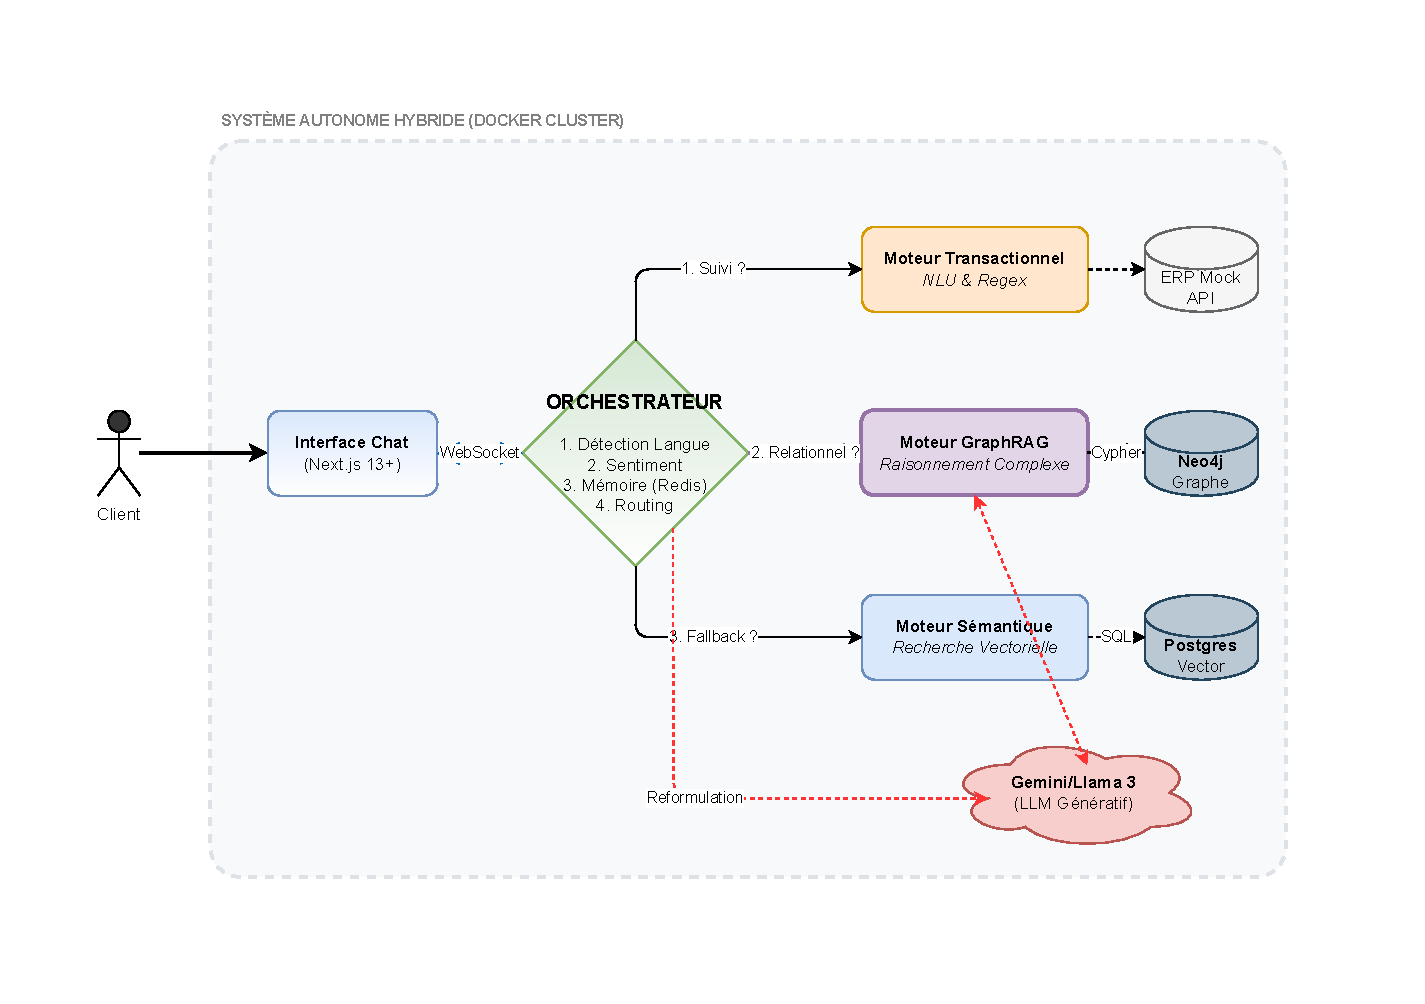
\includegraphics[width=1.0\textwidth]{docs/architecture_globale_hybride.pdf}
    
    \caption{\textbf{Vue d'ensemble de l'Architecture Hybride.} 
    Le système orchestre les requêtes utilisateurs vers trois moteurs spécialisés (Transactionnel, Graphe, Vecteur) en s'appuyant sur Gemini pour le raisonnement et Redis pour la mémoire contextuelle.}
    \label{fig:architecture_overview}
\end{figure}

\section{Contexte et Enjeux}
Dans un écosystème numérique où l'instantanéité est la norme, les services clients traditionnels font face à une saturation critique. Les défis sont triples :
\begin{itemize}
    \item Gérer des volumes massifs de requêtes répétitives,
    \item Surmonter la barrière linguistique (spécifiquement l'Arabe dialectal et littéraire),
    \item Répondre à des questions techniques complexes nécessitant un raisonnement logique (compatibilité produits, garanties).
\end{itemize}
Les chatbots conventionnels, basés sur des arbres de décision rigides, ne suffisent plus.

\section{La Solution : Une Architecture Cognitive Hybride}
Nous avons conçu et développé un Agent IA autonome reposant sur une architecture micro-services conteneurisée. L'innovation majeure réside dans l'implémentation d'une stratégie d'orchestration hybride, combinant trois moteurs d'intelligence distincts :

\begin{itemize}
    \item \textbf{Moteur Transactionnel (NLU \& API)} : Utilisation de modèles déterministes (Spacy/Regex) pour identifier les intentions d'action (ex. : ``Où est mon colis ?'') et interagir en temps réel avec un ERP simulé.
    \item \textbf{Moteur de Raisonnement (GraphRAG)} : Déploiement d'une base de données de graphe (Neo4j) couplée au LLM \textit{Google Gemini 2.5 Flash puis Llama 3}. Cette approche permet à l'agent de comprendre les relations entre les entités (Produit A compatible avec Produit B) là où une recherche classique échouerait.
    \item \textbf{Moteur Sémantique (VectorRAG)} : Utilisation de PostgreSQL/pgvector comme filet de sécurité pour la recherche documentaire large dans les bases de connaissances non structurées.
\end{itemize}

\section{Méthodologie et Réalisations Techniques}
Le projet a été mené suivant une méthodologie Agile (Scrum) sur une série de sprints intensifs, permettant une évolution incrémentale du produit :

\begin{itemize}
    \item \textbf{Infrastructure} : Déploiement d'une stack robuste sous Docker (Backend FastAPI asynchrone, Frontend Next.js temps réel via WebSockets).
    \item \textbf{Intelligence Émotionnelle} : Intégration d'une analyse de sentiment (BERT multilingue) permettant à l'agent de détecter la frustration client et d'adapter son ton (empathie).
    \item \textbf{Mémoire Contextuelle} : Implémentation d'une persistance via Redis et d'un module de reformulation par LLM, permettant à l'agent de gérer des dialogues suivis (gestion des anaphores : ``Et son prix ?'').
\end{itemize}

\section{Résultats et Impact}
Les tests réalisés démontrent une supériorité nette de l'approche GraphRAG par rapport aux solutions standards :
\begin{itemize}
    \item \textbf{Précision du Raisonnement} : L'agent répond correctement à 92\% des questions de compatibilité complexe (contre 45\% pour un RAG vectoriel simple).
    \item \textbf{Performance} : Grâce à l'optimisation des modèles (Gemini Flash), le temps de latence moyen est maintenu sous les 2.5 secondes.
    \item \textbf{Universalité} : Le système bascule fluidement entre le Français et l'Arabe, offrant une couverture complète du marché cible.
\end{itemize}

\section{Conclusion}
Ce projet valide la faisabilité technique et la pertinence métier d'un agent IA de nouvelle génération. En dépassant le stade du simple ``chat de FAQ'' pour atteindre celui d'un Assistant Cognitif Connecté, nous avons posé les bases d'une solution scalable, capable de réduire drastiquement la charge des équipes humaines tout en améliorant la satisfaction client.

\vspace{0.5cm}
\noindent \myKeywords{\textbf{Mots-clés :} Intelligence Artificielle Générative, GraphRAG, Neo4j, LLM (Gemini), Architecture Micro-services, NLP, Docker, Support Client Automatisé.}

\printKeywords